\chapter[Electromagnetic induction and Maxwell's equations]
      [Electromagnetic induction]{Electromagnetic induction and Maxwell's equations}

\section{Faraday's discovery}

{\small
\begin{enumerate}

\item The power which electricity of tension possesses of causing an opposite
electrical state in its vicinity has been expressed by the general term Induction;
which, as it has been received into scientific language, may also, with
propriety, be used in the same general sense to express the power which
electrical currents may possess of inducing any particular state upon matter
in their immediate neighbourhood, otherwise indifferent. It is with this
meaning that I purpose using it in the present paper.

\item Certain effects of the induction of electrical currents have already been
recognised and described: as those of magnetization; Ampere's experiments
of bringing a copper disc near to a flat spiral; his repetition with electromagnets
of Arago's extraordinary experiments, and perhaps a few others.
Still it appeared unlikely that these could be all the effects which induction
by currents could produce; especially as, upon dispensing with iron, almost
the whole of them disappear, whilst yet an infinity of bodies, exhibiting
definite phenomena of induction with electricity of tension, still remain to
be acted upon by the induction of electricity in motion.

\item Further: Whether Ampere's beautiful theory were adopted, or any
other, or whatever reservation were mentally made, still it appeared very
extraordinary, that as every electric current was accompanied by a corresponding
intensity of magnetic action at right angles to the current, good
conductors of electricity, when placed within the sphere of this action, should
not have any current induced through them, or some sensible effect produced
equivalent in force to such a current.

\item These considerations, with their consequence, the hope of obtaining
electricity from ordinary magnetism, have stimulated me at various times
to investigate experimentally the inductive effect of electric currents. I lately
arrived at positive results; and not only had my hopes fulfilled, but obtained
a key which appeared to me to open out a full explanation of Arago's magnetic
phenomena, and also to discover a new state, which may probably have
great influence in some of the most important effects of electric currents.

\item These results I purpose describing, not as they were obtained, but in
such a manner as to give the most concise view of the whole.

\end{enumerate}
}

So begins Michael Faraday's account of the discovery of electromagnetic
induction. This passage was part of a paper Faraday presented
in 1831. It is quoted from his \emph{Experimental Researches in
Electricity}, published in London in 1839. There follows in the paper
a description of a dozen or more experiments, through which Faraday
% p. 227
brought to light every essential feature of the production of electric
efiects by magnetic action.

By ``electricity of tension'' Faraday meant electrostatic charges,
and the induction he refers to in the first sentence involves nothing
more than we have studied in Chap. 3: The presence of a charge
causes a redistribution of charges on conductors nearby. Faraday's
question was, why does not an electric current cause another current
in nearby conductors?

The production of magnetic fields by electric currents had been
thoroughly investigated after Oersted's discovery. The familiar
laboratory source of these ``galvanic'' currents was the voltaic battery.
The most sensitive detector of such currents was a galvanometer. It
consisted of a magnetized needle pivoted like a compass needle or
suspended by a weak fiber between two coils of wire. Sometimes
another needle, outside the coil but connected rigidly to the first
needle, was used to compensate the influence of the earth's magnetic
field (Fig. 7.1a). The sketches in Fig. 7.1b through e represent a
few of Faraday's induction experiments. You must read his own
account, one of the classics of experimental science, to appreciate
the resourcefulness with which he pressed the search, the alert and
open mind with which he viewed the evidence.

In his early experiments Faraday was puzzled to find that a steady
current had no detectable effect on a nearby circuit. He constructed
various coils of wire, of which Fig. 7.1a shows an example, winding
two conductors so that they should lie very close together while still
separated by cloth or paper insulation. One conductor would form
a circuit with the galvanometer. Through the other he would send
a strong current from a battery. There was, disappointingly, no 
deflection of the galvanometer. But in one of these experiments he
noticed a very slight disturbance of the galvanometer when the current
was switched on and another when it was switched off. Pursuing
this lead. he soon established beyond doubt that currents in other
conductors are induced, not by a \emph{steady} current, but by a \emph{changing}
current. One of Faraday's brilliant experimental tactics at this stage
was to replace his galvanometer, which he realized was not a good
detector for a brief pulse of current, by a simple small coil in which
he put an unmagnetized steel needle (Fig. 7.lb). He found that the
needle was left magnetized by the pulse of current induced when the
primary current was switched on---and it could be magnetized in the
opposite sense by the current pulse induced when the primary circuit
was broken.

% p. 228
Here is his own description of another experiment:

\begin{quotation}
In the preceding experiments the wires were placed near to each other.
and the contact of the inducing one with the battery made when the inductive
effect was required; but as the particular action might be supposed to be
exerted only at the moments of making and breaking contact, the induction
was produced in another way. Several feet of copper wire were stretched
in wide zigzag forms, representing the letter W, on one surface of a broad
board; a second wire was stretched in precisely similar forms on a second
board, so that when brought near the first, the wires should everywhere
touch, except that a sheet of thick paper was interposed. One of these wires
was connected with the galvanometer, and the other with a voltaic battery.
The first wire was then moved towards the second, and as it approached, the
needle was deflected. Being then removed, the needle was deflected in the
opposite direction. By first making the wires approach and then recede,
simultaneously with the vibrations of the needle, the latter soon became very
extensive; but when the wires ceased to move from or towards each other,
the galvanometer needle soon came to its usual position.

As the wires approximated, the induced current was in the contrary direction
to the inducing current. As the wires receded, the induced current was
in the same direction as the inducing current. When the wires remained
stationary, there was no induced current.
\end{quotation}

In this chapter we study the electromagnetic interaction that
Faraday explored in those experiments. From our present view-
point, induction can be seen as a natural consequence of the force on
a charge moving in a magnetic field. In a limited sense, we can derive
the Induction Law from what we already know. In following this
course we again depart from the historical order of development, but
we do so (borrowing Faraday's own words from the end of the
passage first quoted) \emph{to give the most concise view of the whole}.

\section[A conducting rod moves through a uniform magnetic field]
      [A conducting rod moves through a magnetic field]{A conducting rod moves through a uniform magnetic field}

Figure 7.2a shows a straight piece of wire, or slender metal rod,
supposed to be moving at constant velocity $\vc{v}$ in a direction perpendicular
to its length. Pervading the space through which the rod
moves there is a uniform magnetic field $\vc{B}$, constant in time. This
could be supplied by a large solenoid enclosing the entire region of
the diagram. The reference frame $\vc{F}$ with coordinates $x$, $y$, $z$ is the
one in which this solenoid is at rest. In the absence of the rod there
is no electric field in that frame, only the uniform magnetic field $\vc{B}$.
The rod, being a conductor, contains charged particles that will
move if a force is applied to them. Any charged particle that is
carried along with the rod, such as the particle of charge $q$ in Fig. 7.2b.
% p. 229
necessarily moves through the magnetic field $\vc{B}$ and does therefore
experience a force
\begin{equation}
  \vc{f} = \frac{q}{c}\vc{v}\times\vc{B}
\end{equation}
With $\vc{B}$ and $\vc{v}$ directed as shown in Fig. 7.2, the force is in the positive
$x$ direction if $q$ is a positive charge, and in the opposite direction for
the negatively charged electrons that are in fact the mobile charge
carriers in most conductors. The consequences will be the same,
whether negatives or positives, or both, are mobile.

When the rod is moving at constant speed and things have settled
down to a steady state, the force $\vc{f}$ given by Eq. 1 must be balanced,
at every point inside the rod, by an equal and opposite force. This
can only arise from an electric field in the rod. The electric field
develops in this way: The force $\vc{f}$ pushes negative charges toward one
end of the rod, leaving the other end positively charged. This goes
on until these separated charges themselves cause an electric field $\vc{E}$
such that, everywhere in the interior of the rod,
\begin{equation}
  q\vc{E} = -\vc{f}
\end{equation}
Then the motion of charge relative to the rod ceases. This charge
distribution causes an electric field outside the rod, as well as inside.
The field outside looks something like that of separated positive and
negative charges with the difference that the charges are not concentrated
entirely at the ends of the rod but are distributed along it. The
external field is sketched in Fig. 7.3a. Figure 7.31) is an enlarged view
of the positively charged end of the rod, showing the charge distribution
on the surface and some field lines both outside and inside the
conductor. That is the way things look, at any instant of time, in
frame $F$.

Let us observe this system from a frame $F'$ that moves with the rod.
Ignoring the rod for the moment, we see in this frame $F'$, indicated in
Fig. 7.2c, a magnetic field $\vc{B}'$ (not much different from $\vc{B}$ if $v$ is small)
together with a uniform electric field, as given by Eq. 6.62,
\begin{equation}
  \vc{E}' = -\frac{\vc{v}'}{c}\times\vc{B}' = \frac{\vc{v}}{c}\times\vc{B}'
\end{equation}
When we add the rod to this system, all we are doing is putting a
stationary conducting rod into a uniform electric field. There will
be a redistribution of charge on the surface of the rod so as to make
the electric field zero inside, as in the case of the metal box of Fig. 3.6,
% p. 230
or of any other conductor in an electric field. The presence of the
magnetic field $\vc{B}'$ has no influence on this static charge distribution.
Figure 7.4a shows some electric field lines in the frame $F'$, and in the
magnified view of the end of the rod in Fig. 7.4b we observe that the
electric field inside the rod is zero.

Except for the Lorentz contraction, which is second order in $v/c$
the charge distribution seen at one instant in frame F, Fig. 7.31:, is the
same as that seen in $F'$. The electric fields differ because the field in
Fig. 7.3 is that of the surface charge distribution alone, while the
electric field we see in Fig. 7.4 is the field of the surface charge
distribution plus the uniform electric field that exists in that frame
of reference. An observer in $F$ says: ``Inside the rod there has developed
an electric field $\vc{E} = - (\vc{v}/c) \times \vc{B}$, exerting a force 
$q\vc{E}=-q(\vc{v}/c)\times\vc{B}$
which just balances the force $q(\vc{v}/c) \times \vc{B}$ that would
otherwise cause any charge $q$ to move along the rod.'' An observer
in $F'$ says: ``Inside the rod there is no electric field, and although there
is a uniform magnetic field here, no force arises from it because no
charges are moving.'' Each account is correct.

% p. 232
\section{A loop moves through a nonuniform magnetic field}

What if we made a rectangular loop of wire, as shown in Fig. 7.5,
and moved it at constant speed through the uniform field $\vc{B}$? To
predict what will happen, we need only ask ourselves---adopting the
frame $F'$---what would happen if we put such a loop into a uniform
electric field. Obviously two opposite sides of the rectangle would
acquire some charge, but that would be all. Suppose, however, that
the field $\vc{B}$ in the frame $F$, though constant in time, is \emph{not uniform} in
space. To make this vivid, we show in Fig. 7.6 the field $\vc{B}$ with a short
solenoid as its source. This solenoid, together with the battery that
supplies its constant current, is fixed near the origin in the frame $F$.
(We said earlier there is no electric field in $F$; if we really use a
solenoid of finite resistance to provide the field, there will be an electric
field associated with the battery and this circuit. It is irrelevant
to our problem and can be ignored. Or we can pack the whole
solenoid, with its battery, inside a metal box.)

Now, with the loop moving with speed $v$ in the $y$ direction, in the
frame $F$, let its position at some instant $t$ be such that the magnetic
field strength is $B_1$ at the left side of the loop and $B_2$ along the right
side (Fig. 7.6). Let $\vc{f}$ denote the force which acts on a charge $q$ that
rides along with the loop. This force is a function of position on the
loop, at this instant of time. Let's evaluate the line integral of $\vc{f}$,
taken around the whole loop: On the two sides of the loop which lie
parallel to the direction of motion, $\vc{f}$ is perpendicular to the path
% p. 233
element $\der\vc{s}$, so these give nothing. Taking account of the contributions
from the other two sides, each of length $w$, we have:
\begin{equation}
  \int \vc{f}\cdot\der\vc{s} = \frac{qv}{c}(B_1-B_2)w
\end{equation}

If we imagine a charge $q$ to move all around the loop, in a time
short enough so that the position of the loop has not changed ap-
preciably, then Eq. 4 gives the work done by the force $\vc{f}$. The work
done \emph{per unit charge} is $(1/q)\int\vc{f}\cdot\der\vc{s}$.
We call this quantity \emph{electromotive force}.\index{electromotive force!generalized definition}
We use the symbol $\emf$ for it, and often shorten the name
to ``emf.'' $\emf$ has the same dimensions as electric potential and is
measured in statvolts, or ergs per unit charge, in the CGS system.
\begin{equation}
  \emf = \frac{1}{q}\int\vc{f}\cdot\der\vc{s}
\end{equation}
The term \emph{electromotive force} was introduced earlier, in Sec. 4.10. It
was defined as the work per unit charge involved in moving a charge
around a circuit containing a voltaic cell. We now broaden the
definition of emf to include any influence that causes charge to
circulate around a closed path. If the path happens to be a physical
circuit with resistance $R$, then the emf $\emf$ will cause a current to flow
according to Ohm's law: $I = \emf/R$. In the particular case we are considering,
$\vc{f}$ is the force that acts on a charge moving in a magnetic
field, and $\emf$ has the magnitude:
\begin{equation}
  \emf = \frac{vw}{c}(B_1-B_2)
\end{equation}
The electromotive force given by Eq. 6 is related in a very simple way
to the \emph{rate of change of magnetic flux through the loop}. By the magnetic
flux through a loop we mean the surface integral of $\vc{B}$ over a
surface which has the loop for its boundary. The flux $\Phi$ through the
closed curve or loop C in Fig. 7.7a is given by the surface integral
of $\vc{B}$ over $S_1$:
\begin{equation}
  \Phi_{(S_1)} = \int_{S_1} \vc{B}\cdot\der\vc{a}_1
\end{equation}

We could draw infinitely many surfaces bounded by $C$. Figure 7.7b
shows another one, $S_2$. Why don't we have to specify which surface
to use in computing the flux? It \emph{doesn't make any difference} because
$\int\vc{B}\cdot\der\vc{a}$ will have the same value for all such surfaces. Let's take a
minute to settle this point once and for all. The flux through $S_2$ will
be $\int_{S_2} \vc{B}\cdot\der\vc{a}_2$. Notice that we let the vector $\der\vc{a}_2$ stick out from the
% p. 234
upper side of $S_2$, to be consistent with our choice of side of $S_1$. This
will give a positive number if the net flux through $C$ is upward.
\begin{equation}
  \Phi_{(S_2)} = \int_{S_2} \vc{B}\cdot\der\vc{a}_2
\end{equation}
We learned in Sec. 6.2 that the magnetic field has zero divergence:
$\div\vc{B}$ = 0. It follows then from Gauss's theorem that if $S$ is any
\emph{closed} surface (``balloon''), and $V$ is the volume inside it:
\begin{equation}
  \int_S \vc{B}\cdot\der\vc{a} = \int_V \div\vc{B}\der v = 0
\end{equation}
Apply this to the closed surface, rather like a kettle drum, formed by
joining our $S_1$ and $S_2$, as in Fig. 7.7c. On $S_2$ the outward normal is
opposite to the vector $\der\vc{a}_2$ we used in calculating the flux through $C$.
Thus
\begin{align}
\begin{split}
  0 &= \int_S \vc{B}\cdot\der\vc{a} = \int \vc{B}\cdot\der\vc{a}_1+\int \vc{B}\cdot(-\der\vc{a}_2) \\
\intertext{or}
    & \int_{S_1} \vc{B}\cdot\der\vc{a}_1 =   \int_{S_2} \vc{B}\cdot\der\vc{a}_2
\end{split}
\end{align}
This shows that it doesn't matter which surface we use to compute
the flux through $C$.

This is all pretty obvious if you realize that $\div\vc{B}$ = 0 implies a
kind of spatial conservation of flux. As much flux enters any volume
as leaves it. (We are considering the situation in the whole space at
one instant of time.) It is often helpful to visualize ``tubes'' of flux.
A flux tube (Fig. 7.8) is a surface at every point on which the magnetic
field line lies in the plane of the surface. It is a surface through
which no flux passes, and we can think of it as containing a certain
amount of flux, as a telephone cable contains wires. Through any
closed curve drawn tightly around a flux tube, the same flux passes.
This could be said about the electric field $\vc{E}$ only for regions where
there is no electric charge, since $\div\vc{E} = 4\pi\rho$. The magnetic field
always has zero divergence everywhere.

Returning now to the moving rectangular loop, let us find the \emph{rate
of change} of flux through the loop. In time $\der t$ the loop moves a distance
$v\;\der t$. This changes in two ways the total flux through the loop,
which is $\int\vc{B}\cdot\der\vc{a}$ over a surface spanning the loop. As you can see
in Fig. 7.9, flux is gained at the right, in amount $B_2 wv\der t$, while an
amount of flux $B_1 wv\der t$ is lost at the left. Hence $\der\Phi$, the change in
flux through the loop in time $\der t$, is
\begin{equation}
  \der\Phi = -(B_1-B_2)wv\der t
\end{equation}
% p. 235
Comparing Eq. 11 with Eq. 6, we see that, in this case at least, the
electromotive force can be expressed as:
\begin{equation}
  \emf = -\frac{1}{c}\frac{\der\Phi}{\der t}
\end{equation}
We can show that this holds quite generally, for a loop of any shape
moving in any manner. The loop $C$ in Fig. 7.10 occupies the position
$C_1$ at time $t$, and it is moving so that it occupies the position $C_2$ at
time $t + \der t$. A particular element of the loop $\der s$ has been transported
with velocity $\vc{v}$ to its new position. $S$ indicates a surface that spans
the loop at time $t$. The flux through the loop at this instant of time is
\begin{equation}
  \Phi(t) = \int_S\vc{B}\cdot\der\vc{a}
\end{equation}
The magnetic field $\vc{B}$ comes from sources that are stationary in our
frame of reference and remains constant in time, at any point fixed
in this frame. At time $t + \der t$ a surface which spans the loop is the
original surface $S$, left fixed in space, augmented by the ``rim'' $\der S$.
(Remember, we are allowed to use \emph{any} surface spanning the loop to
compute the flux through it.) Thus:
\begin{equation}
  \Phi(t+\der t) = \int_{S+\der S} \vc{B}\cdot\der\vc{a} = \Phi(t)+\int_{\der S}\vc{B}\cdot\der\vc{a}
\end{equation}
Hence the change in flux, in time $\der t$, is just the flux through the ``rim''
$\der S$, $\int_{\der S}\vc{B}\cdot\der\vc{a}$. On the rim, an element of surface area da can be 
expressed as $(\vc{v} \der t) \times \der\vc{s}$, so the integral over the surface $\der S$ can be
written as an integral around the path $C$, in this way:
\begin{equation}
  \der\Phi = \int_{\der S}\vc{B}\cdot\der\vc{a} = \int_C \vc{B}\cdot[(\vc{v}\der t)\times\der\vc{s}]
\end{equation}
Since $\der t$ is a constant for the integration, we can factor it out and
have:
\begin{equation}
  \frac{\der\Phi}{\der t} = \int_C \vc{B}\cdot(\vc{v}\times\der\vc{s})
\end{equation}
According to the rule for the scalar triple product (Vol. I, p. 38,
Eq. 52) we have the identity: $\vc{a}\cdot (\vc{b} \times \vc{c}) = - (\vc{b} \times \vc{a}) \cdot \vc{c}$.
Using this to rearrange the integrand in Eq. 16, we have:
\begin{equation}
  \frac{\der\Phi}{\der t} = - \int_C (\vc{v}\times\vc{B})\cdot\der\vc{s}
\end{equation}
% p. 236
Now the force on a charge $q$ which is carried along by the loop is just
$q(\vc{v} \times \vc{B}) /c$, so the electromotive force, which is the line integral
around the loop of the force per unit charge, is just
\begin{equation}
  \emf = \frac{1}{c} \int_C (\vc{v}\times\vc{B})\cdot\der\vc{s}
\end{equation}
Comparing Eq. 17 with Eq. 18 we get the simple relation already
given in Eq. 12, but valid now for arbitrary shape and motion of the
loop. (We did not even have to assume that $\vc{v}$ is the same for all
parts of the loop!) In summary, the line integral around a moving
loop of $\vc{f}/q$, the force per unit charge, is just $-1/c$ times the rate of
change of flux through the loop.

The sense of the line integral and the direction in which flux is
called positive are to be related by a right-hand-thread rule. For
instance, in Fig. 7.6, the flux is \emph{upward} through the loop and is
\emph{decreasing}. Taking the minus sign in Eq. 12 into account, our rule
would predict an electromotive force which would tend to drive a
positive charge around that loop in a counterclockwise direction, as
seen looking down on the loop (Fig. 7.11).

There is a better way to look at this question of sign and direction.
Notice that if a current should flow in the direction of the induced
electromotive force, in the situation shown in Fig. 7.11, this current
itself would create some flux through the loop in a direction to
\emph{counteract} the assumed flux change. That is an essential physical
fact, and not the consequence of an arbitrary convention about signs
and directions. It is a manifestation of the tendency of systems to
resist change. In this context it is traditionally called Lenz's law.

Another example of Lenz's law is illustrated in Fig. 7.12. The
conducting ring is falling in the magnetic field of the coil. The flux
through the ring is \emph{downward} and is \emph{increasing} in magnitude. To
counteract this change, some new flux upward is needed. It would
take a current flowing around the ring in the direction of the arrows
to produce such flux. Lenz's law assures us that the induced emf will
be in the right direction to cause such a current.

If the electromotive force causes current to flow in the loop which
is shown in Figs. 7.6 and 7.11, as it will if the loop has a finite resist-
ance, some energy will be dissipated in the wire. What supplies this
energy? To answer that, consider the force that acts on the current
in the loop if it flows in the sense indicated by the arrow in Fig. 7.11.
The conductor on the right, in the field $B_2$, will experience a force
toward the right, while the opposite side of the loop, in the field $B_1$,
% p. 237
will be pushed toward the left. But $B_1$ is greater than $B_2$, so the net
force on the loop is toward the left, \emph{opposing the motion}. To keep
the loop moving at constant speed some external agency has to do
work, and the energy thus invested eventually shows up as heat in
the wire. Imagine what would happen if Lenz's law were violated,
or if the force on the loop were to act in a direction to assist the
motion of the loop!

A very common element in electrical machinery and electrical instruments
is a loop or coil that rotates in a magnetic field. Let's apply
what we have just learned to the system shown in Fig. 7.13, a single
loop rotating at constant speed in a magnetic field that is approximately
uniform. The mechanical essentials, shaft, bearings, drive,
etc., are not drawn. The field $\vc{B}$ is provided by the two fixed coils.
Suppose the loop rotates with angular velocity $\omega$ in radians/sec. If
its position at any instant is specified by the angle $\theta$, then $\theta=\omega t +\alpha$,
% p. 238
where the constant $\alpha$ is simply the position of the loop at $t = 0$. The
component of $\vc{B}$ perpendicular to the plane of the loop is $B \sin \theta$.
Therefore the flux through the loop at time $t$ is
\begin{equation}
  \Phi(t) = SB\sin(\omega t+\alpha)
\end{equation}
where $S$ is the area of the loop. For the induced electromotive force
we then have: 
\begin{equation}
  \emf = -\frac{1}{c}\frac{\der\Phi}{\der t} = -\frac{SB\omega}{c} \cos(\omega t+\alpha)
\end{equation}
If the loop instead of being closed is connected through slip rings to
external wires, as shown in Fig. 7.13, we can detect at these terminals
a sinusoidally alternating potential difference.

A numerical example may clear up any question about units.
Suppose the magnetic field strength $B$ is 500 gauss, the speed of rotation
30 revolutions per second, the loop area $100\ \cmunit^2$. Then
$\omega = 2\pi \times 30$, or 188 radians/sec, and the amplitude, that is, the
maximum magnitude, of the oscillating electromotive force is
\begin{align}
\begin{split}
  \emf_{\text{max}} &= \frac{SB\omega}{c} 
        = \frac{(188\ \sunit^{-1})(100\ \cmunit^2)(500\ \text{gauss})}{(3\times10^{10}\ \cmunit/\sunit)} \\
        &= 3.1\times10^{-4}\ \text{gauss}\cdot\cmunit,\ \text{or statvolt}
\end{split}
\end{align}
Since $\emf$ is work per unit charge, it ought to come out in statvolts in
the CGS system we are using. Notice that the units in Eq. 21 reduce
to gauss-centimeters. Electric field strength $\vc{E}$ and magnetic field
strength $B$ have the same dimensions in the Gaussian CGS system.
For instance, in a transformation formula like $\vc{E}' = (v/c) \times \vc{B}$, we
multiply a magnetic field strength by the dimensionless ratio $v/c$ to
obtain an electric field strength. (The unit of electric field strength,
statvolts per centimeter, happens not to have been given a name all
its own, like \emph{gauss}.) Thus $1\ \zu{gauss}\cdot\cmunit$ translates directly to 
$1\ (\text{statvo1t}/\cmunit)\cdot\cmunit$, that is, 1 statvolt. In ordinary volts, the ``practical''
unit, the amplitude of the electromotive force in this example
amounts to $3.1 \times 10^{-4} \times 300$, or 0.093 volt.

\section{A stationary loop with the field source moving}

We can, if we like, look at the events depicted in Fig. 7.6 from a
frame of reference that is moving with the loop. That can't change
the physics, only the words we use to describe it. Let $F'$, with coordinates
$x'$, $y'$, $z'$, be the frame attached to the loop, which we now regard
% p. 239
as stationary (Fig. 7.14). The coil and battery, stationary in frame $F$,
are moving in the $-y'$ direction with velocity $\vc{v}' = -\vc{v}$. Let $B'_1$ and
$B'_2$ be the magnetic fields measured at the two ends of the loop by
observers in $F'$ at some instant $t'$. At these positions there will be
an electric field in $F'$. Equation 6.62 tells us that
\begin{align}
\begin{split}
  \vc{E}'_1 &= -\frac{\vc{v'}\times\vc{B}_1'}{c} = \frac{\vc{v}\times\vc{B}'_1}{c} \\
  \vc{E}'_2 &= -\frac{\vc{v'}\times\vc{B}_2'}{c} = \frac{\vc{v}\times\vc{B}'_2}{c} 
\end{split}
\end{align}
For observers in $F'$ this is a genuine electric field. It is not an
electrostatic field. The line integral of $\vc{E}'$ around any closed path in
$F'$ is not generally zero. In fact, the line integral of $\vc{E}'$ around the
rectangular loop is:
\begin{equation}
  \int \vc{E}'\cdot\der\vc{s}' = \frac{wv}{c}(B'_1-B'_2)
\end{equation}

We can call the line integral in Eq. 23 the electromotive force $\emf'$ on
this path. If a charged particle moves once around the path, $\emf'$ is
the work done on it, per unit charge. $\emf'$ is related to the rate of
% p. 240
change of flux through the loop. To see this, note that while the loop
itself is stationary, the \emph{magnetic field pattern} is now moving with the
velocity $-\vc{v}$ of the source. Hence for the flux lost or gained at either
end of the loop, in a time interval $\der t'$, we get a result similar to Eq. 11,
and we conclude that
\begin{equation}
  \emf' = \frac{1}{c}\frac{\der\Phi'}{\der t'}
\end{equation}

We can summarize as follows the descriptions in the two frames of
reference, $F$, in which the source of $\vc{B}$ is at rest, and $F'$, in which the
loop is at rest:

An observer in $F$ says, ``We have here a magnetic field which,
though it is not uniform spatially, is constant in time. There is no
electric field. That wire loop over there is moving with velocity $\vc{v}$
through the magnetic field, so the charges in it are acted on by a force
$(\vc{v}/ c) \times \vc{B}$ dynes per unit charge. The line integral of this 
force-per-unit-charge, taken around the whole loop is the electromotive force $\emf$
and it is equal to $-(1/c)(\der\Phi/\der t)$. The flux $\Phi$ is $\int\vc{B}\cdot\der\vc{a}$ over a surface
$S$ which, at some instant of time $t$ by my clock, spans the loop.''

An observer in $F'$ says, ``This loop is stationary and only an electric
field could cause the charges in it to move. But there is in fact an
electric field $\vc{E}'$. It seems to be caused by that magnetlike object
which happens at this moment to be whizzing by with a velocity $-\vc{v}$,
producing at the same time a rather strong magnetic field $\vc{B}'$. The
electric field is such that $\int\vc{E}'\cdot\der\vc{s}'$ around this stationary loop is not
zero but instead is equal to $-1/c$ times the rate of change of flux
through the loop, $\der\Phi'/\der t'$. The flux $\Phi'$ is $\int\vc{B}'\cdot\der\vc{a}'$ over a surface
spanning the loop, the values of $B'$ to be measured all over this surface
at some one instant $t'$, by my clock.''

Our conclusions so far are relativistically exact. They hold for
any speed $v \le c$ provided we observe scrupulously the distinctions
between $\vc{B}$ and $\vc{B}'$, $t$ and $t'$, etc. If $v \ll c$, so that $v^2/c^2$ can be
neglected, $B'$ will be practically equal to $B$, and we can safely ignore
also the distinction between $t$ and $t'$.

\section{A universal law of induction}

Let's carry out three experiments with the apparatus shown in
Fig. 7.15. The tables are on wheels so that they can be easily moved.
A sensitive galvanometer has been connected to our old rectangular
loop, and to increase any induced electromotive force we put several
turns of wire in the loop rather than one. Frankly though, our
% p. 241
sensitivity might still be marginal, with the feeble source of magnetic
field pictured. Perhaps you can devise a more practical version of
the experiment in the laboratory.

\begin{description}

\item[\textbf{Experiment I}.] With constant current in the coil and table 1 
stationary, table 2 moves toward the right at speed $v$. \emph{The galvanometer
deflects.} We are not surprised; we have already analyzed this situation
in Sec. 7.3 above.

\item[\textbf{Experiment II}.] With constant current in the coil and table 2 
stationary, table 1 moves to the left with speed $v$. \emph{The galvanometer
deflects.} This doesn't surprise us either. We have just discussed the
equivalence of Experiments I and II, an equivalence which is an example
of Lorentz invariance or, for the low speeds of our tables,
Galilean invariance. We know that in both experiments the deflection
of the galvanometer can be related to the rate of change of flux
of $\vc{B}$ through the loop.

\item[\textbf{Experiment III}.] Both tables remain at rest, but we vary the current
$I$ in the coil by sliding the contact $K$ along the resistance strip. We
do this in such a way that the \emph{rate of decrease} of the field $\vc{B}$ at the loop
is the same as it was in Experiments I and II. \emph{Does the galvanometer
deflect?}

\end{description}

% p. 242

For an observer stationed at the loop on table 2 and measuring
the magnetic field in that neighborhood as a function of time and
position, there is no way to distinguish between Experiments I, II,
and III. Imagine a black cloth curtain between the two tables.
Although there might be minor differences between the field configurations
for II and III, an observer who did not know what was
behind the curtain could not decide, on the basis of local $\vc{B}$ measurements
alone, which case it was. Therefore if the galvanometer did
not respond with the same deflection in Experiment III, it would
mean that the relation between the magnetic and electric fields in a
region depends on the nature of a remote source. Two magnetic
fields essentially similar in their local properties would have associated
in one case, but not in the other, an electric field with
$\int\vc{E}\cdot\der\vc{s}\ne0$.

We find by experiment that III \emph{is} equivalent to I and II. The
galvanometer defiects, by the same amount as before. Faraday's
experiments were the first to demonstrate this fundamental fact.
The electromotive force we observe depends only on the rate of
change of the flux of $\vc{B}$, and not on anything else. We can state as a
universal relation Faraday's Law of Induction:\index{induction!Faraday's law of}\index{Faraday!law of induction}

\begin{framed}
If $C$ is some closed curve, stationary in coordinates
$x$, $y$, $z$, if $S$ is a surface spanning $C$, and $\vc{B}(x,y,z,t)$ is the
magnetic field measured in $x$, $y$, $z$, at any time $t$, then
\begin{equation}
  \emf = \int_C \vc{E}\cdot\der\vc{s} = -\frac{1}{c}\frac{\der}{\der t}\int_S \vc{B}\cdot\der\vc{a}
       = -\frac{1}{c}\frac{\der\Phi}{\der t}
\end{equation}
\end{framed}

Using the vector derivative curl, we can express this law in differential
form. If the relation
\begin{equation}
  \int_C \vc{E}\cdot\der\vc{s} = -\frac{1}{c}\frac{\der}{\der t}\int_S \vc{B}\cdot\der\vc{a}
\end{equation}
is true for \emph{any} curve $C$ and spanning surface $S$, as our law asserts, it
follows that at any point
\begin{equation}
  \curl\vc{E} = -\frac{1}{c}\frac{\der\vc{B}}{\der t}
\end{equation}
To show that Eq. 27 follows from Eq. 26, we proceed as usual to let $C$
shrink down around a point, which we take to be a nonsingular
point for the function $\vc{B}$. Then in the limit the variation of $\vc{B}$ over the
% p. 243
small patch of surface $\vc{a}$ that spans $C$ will be negligible and the surface
integral will approach simply $\vc{B}\cdot\vc{a}$. Now by definition (Eq. 2.76)
the limit approached by $\int_C\vc{E}\cdot\der\vc{s}$ as the patch shrinks is $\vc{a}\cdot\curl\vc{E}$.
Thus we have, in the limit,
\begin{equation}
  \vc{a}\cdot\curl\vc{E} = -\frac{1}{c}\frac{\der}{\der t}(\vc{B}\cdot\vc{a})
        = \vc{a}\cdot\left(-\frac{1}{c}\frac{\der\vc{B}}{\der t}\right)
\end{equation}
Since this holds for \emph{any} infinitesimal $\vc{a}$,
it must be that\footnote{If that isn't obvious, note that choosing $\vc{a}$ in the $x$
direction will establish that
$(\curl\vc{E})_x = -\frac{1}{c}\frac{\der B_x}{\der t}$, and so on.}
\begin{equation}
  \curl\vc{E} = -\frac{1}{c}\frac{\der\vc{B}}{\der t}
\end{equation}
Recognizing that $\vc{B}$ may depend on position as well as time we shall
write $\partial\vc{B}/\partial t$ in place of $\der \vc{B}/\der t$. We have then these two entirely
equivalent statements of the law of induction:
\begin{framed}
\begin{align}
  \int_C \vc{E}\cdot\der\vc{s} &= -\frac{1}{c}\frac{\der}{\der t}\int_S \vc{B}\cdot\der\vc{a} \\
\intertext{or}
  \curl\vc{E} = -\frac{1}{c}\frac{\partial\vc{B}}{\partial t}
\end{align}
\end{framed}
In Eq. 30 the electric field $\vc{E}$ is to be expressed in absolute electrostatic
units, that is, statvolts per centimeter, and $\vc{B}$ is to be measured
in gauss. The electromotive force $\emf = \int_C \vc{E}\cdot\der\vc{s}$ will be given in statvolts.
In practical calculations we often prefer to express electromotive
force in volts, while retaining gauss for the unit of magnetic
field strength. Recalling that l statvolt is equivalent to 300 volts,
we see that the relation between $\emf$ and the rate of change of flux
must be:
\begin{align}
\begin{split}
  \underbrace{\emf}_\text{(volts)} 
  &= \int_C \underbrace{\vc{E}}_\text{(volts/cm)}\cdot\underbrace{\der\vc{s}}_\text{(cm)} \\
  &= -(10^{-8}) \underbrace{\frac{\der}{\der t}}_\text{($\sunit^{-1}$)}
    \int \underbrace{\vc{B}}_\text{(gauss)}
    \cdot \underbrace{\der\vc{a}}_\text{($\cmunit^2$)} \\
  &= -(10^{-8})\frac{\der\Phi}{\der t} \qquad \left(\frac{\zu{gauss}\cdot\cmunit^2}{\sunit}\right)
\end{split}
\end{align}
The differential expression, $\curl\vc{E} = - (1/c) \partial\vc{B}/\partial t$, brings out
rather plainly the point we tried to make earlier about the local nature
% p. 244
of the field relations. The variation in time of $\vc{B}$ in a neighborhood
completely determines $\curl\vc{E}$ there --- nothing else matters. That
does not completely determine $\vc{E}$ itself, of course. Without affecting
this relation any electrostatic field, with $\curl\vc{E} = 0$, could be
superposed.

As a concrete example, suppose coils like those in Fig. 7.13 are
supplied with 60 cycle/s alternating current, instead of direct
current. The current and the magnetic field vary as $\sin (2\pi\cdot 60\cdot t)$,
or $\sin 377t$. Suppose the amplitude of the current is such that the
magnetic field $\vc{B}$ in the central region reaches a maximum value of
50 gauss. We want to investigate the induced electric field, and the
electromotive force, on the circular path $10\ \cmunit$ in radius shown in
Fig. 7.16. We may assume that the field $B$ is practically uniform in
the interior of this circle, at any instant of time.
\begin{equation}
  B = 50 \sin 377t
\end{equation}
% p. 245
$B$ is in gauss and $t$ in seconds. The flux through the loop $C$ is
\begin{align}
  \Phi &= \pi r^2 B = \pi \times 10^2 \times 50\sin 377 t \\
       &= 15,700 \sin 377 t \qquad \text{($\zu{gauss}\cdot\cmunit^2$)}
\end{align}

Using Eq. 31 to calculate the electromotive force in volts,
\begin{align}
  \emf &= -(10^{-8})\frac{\der\Phi}{\der t} = -(10^{-8})(377)(15,700)\;\cos 377 t \\
       &= -0.059\cos 377 t \qquad \text{(volts)}
\end{align}
The maximum attained by $\emf$ is 59 millivolts. The minus sign will
ensure that Lenz's law is respected, if we have defined our directions
consistently. The variation of both $\Phi$ and $\emf$ with time is shown in
Fig. 7.17.

What about the electric field itself? Usually we cannot deduce
$\vc{E}$ from a knowledge of $\curl\vc{E}$ alone. However, our path $C$ is here a
circle around the center of a symmetrical system. \emph{If there are no
other} electric fields around, we may assume that on the circle $C$, $\vc{E}$ lies
in that plane and has a constant magnitude. Then it is a trivial
matter to predict its magnitude, since $\int_C \vc{E}\cdot\der\vc{s} = 2\pi r E = \emf$, which
we have already calculated. In this case, the electric field on the
circle might look like Fig. 7.18a at a particular instant. But if there
are other field sources it could look quite different. If there happened
to be a positive and a negative charge located on the axis as shown
in Fig. 7.18b, the electric field in the vicinity of the circle would be
the superposition of the electrostatic field of the two charges and the
induced electric field.

% p. 246

\section{Mutual inductance}

Two circuits, or loops, $C_1$ and $C_2$ are fixed in position relative to
one another (Fig. 7.19). By some means, such as a battery and
a variable resistance, a controllable current $I_1$ is caused to flow in
circuit $C_1$. Let $\vc{B}_1(x,y,z)$ be the magnetic field that would exist if
the current in $C_1$ remained constant at the value $I_1$, and let $\Phi_{21}$ denote
the flux of $\vc{B}_1$ through the circuit $C_2$. Thus,
\begin{equation}
  \Phi_{21} = \int_{S_2} \vc{B}\cdot\der\vc{a}_2
\end{equation}
where $S_2$ is a surface spanning the loop $C_2$. With the shape and
relative position of the two circuits fixed, $\Phi_{21}$ will be proportional
to $I_1$:
\begin{equation}
  \frac{\Phi_{21}}{I_1} = \text{const}
\end{equation}

Suppose now that $I_1$ changes with time, but \emph{slowly enough} so that
the field $\vc{B}_1$ at any point in the vicinity of $C_2$ and the current $I_1$ in $C_1$
at the same instant of time are related as they would be for steady
currents. (To see why such a restriction is necessary, imagine that $C_1$
and $C_2$ are 10 meters apart and we cause the current in $C_1$ to double in
value in 10 nanoseconds!) The flux $\Phi_{21}$ will change in proportion
as $I_1$ changes. There will be an electromotive force induced in
circuit $C_2$, of magnitude
\begin{equation}
  \emf_{21} = -\frac{\text{const}}{c} \frac{\der I_1}{\der t}
\end{equation}
% p. 247
The constant here is the same as the one in Eq. 36. Let's absorb the
$c$ in the denominator into a single constant, denoted by $M_{21}$, and write
Eq. 37 in this way:
\begin{equation}
  \emf_{21} = -M_{21} \frac{\der I_1}{\der t}
\end{equation}

We call the constant $M_{21}$ the coefficient of \intro{mutual inductance}. Its
value is determined by the geometry of our arrangement of loops.
The units will of course depend on our choice of units for $\emf$, $I$, and $t$.
In the practical system, with $\emf_{21}$ in volts and $I_1$ in amperes, $M$ is expressed
in\index{henry (unit)} \emph{henrys}.\footnote{The unit is named after 
Joseph Henry (1797-1878), the foremost American physicist\index{Henry, Joseph}
of his time. Electromagnetic induction was discovered independently by Henry, practically
at the same time as Faraday's experiments. Henry was the first to recognize the
phenomenon of self-induction. He developed the electromagnet and the prototype of
the electric motor, invented the electric relay, and all but invented telegraphy.}
That is, the mutual inductance $M_{21}$ is one henry
if a current $I_1$ changing at the rate of $1\ \text{ampere}/\sunit$ induces an electromotive
force of 1 volt in circuit $C_2$.

As an example, consider the circuits in Fig. 7.20, two coplanar,
concentric rings, a small ring $C_2$ and a much larger ring $C_1$. What
is $M_{21}$ in this case? At the center of $C_1$, with $I_1$ flowing, the field $B_1$
is given by
\begin{equation}
  B_1 = \frac{2\pi I_1}{c R_1}
\end{equation}
with $I_1$ in $\esu/\sunit$, $B_1$ in gauss. (Review the paragraph at the beginning
of Sec. 6.5, leading to Eq. 6.42, if you don't remember how to
find the field at the center of a current ring.) We assume $R_2 \ll R_1$
so that we can neglect the variation of $B_1$ over the interior of the small
ring. Then the flux through the small ring is
\begin{equation}
  \Phi_{21} = (\pi R_2^2)\frac{2\pi I_1}{c R_1} = \frac{2\pi^2 I_1 R_2^2}{c R_1}
\end{equation}
Thus the ``constant'' in Eq. 36, in this particular case, has the value
$2\pi^2R_2^2/cR_1$, and the electromotive force induced in $C_2$ will be
\begin{equation}
  \emf_{21} = -\frac{1}{c}\cdot\frac{2\pi^2 R_2^2}{c R_1}\cdot \frac{\der I_1}{\der t}
\end{equation}
% p. 248
with $\emf_{21}$ in statvolts and $I_1$ in esu per second. To express the mutual
inductance in henrys, we note that a statvolt is 300 volts and
$I(\esu/\sunit) = I(\text{amperes}) \times 3 \times 10^9$, so that
\begin{equation}
  \emf (\text{volts}) = - \frac{2\pi^2 R_2^2}{ R_1} \times 10^{-9} \frac{\der I}{\der t}\qquad(\text{amperes/s})
\end{equation}
Thus the value of $M_{21}$ in henrys, with $R_2$ and $R_1$ in centimeters, is
\begin{equation}
  M_{21} = \frac{2\pi^2 \times 10^{-9}R_2^2}{R_1}
\end{equation}
Incidentally, the minus sign we had been carrying along doesn't tell
us much at this stage. If you want to be sure which way the electromotive
force will tend to drive current in $C_2$, Lenz's law is your most
reliable guide.

If the circuit $C_1$ consisted of $N_1$ turns of wire instead of a single
ring, the field $B_1$ at the center would be $N_1$ times as strong, for a given
current $I_1$. Also, if the small loop $C_2$ consisted of $N_2$ turns, all of the
same radius $R_2$, the electromotive force in each turn would add to
that in the next, making the total electromotive force in that circuit
$N_2$ times that of a single turn. Thus for \emph{multiple turns} in each coil
the mutual inductance will be given by
\begin{equation}
  M_{21} = \frac{2\pi^2 \times 10^{-9}N_1N_2R_2^2}{R_1}
\end{equation}
This assumes that the turns in each coil are neatly bundled 
together, the cross section of the bundle being small compared to the
coil radius. However, the mutual inductance $M_{21}$ has a well-defined
meaning for two circuits of any shape or distribution. It is the ratio
of the electromotive force in volts in circuit 2, caused by changing
current in circuit 1, to the rate of change of current $I_1$ in amperes/second.
That is,
\begin{equation}
  M_{21}(\text{henrys})
        = \frac{\emf_{21}\ (\text{volts})}{\left(\frac{\der I_1}{\der t}\right)\left(\frac{\text{A}}{s}\right)}
\end{equation}

% p. 249

\section{A ``reciprocity'' theorem}

In considering the circuits $C_1$ and $C_2$ we might have inquired about
the electromotive force induced in circuit $C_1$ by a changing current
in circuit $C_2$. That would involve another coefficient of mutual
inductance, $M_{12}$:
\begin{equation}
  M_{12} = \frac{\emf_{12}}{\left(\frac{\der I_2}{\der t}\right)}
\end{equation}
It is a remarkable fact that for \emph{any} two circuits,
\begin{equation}
  M_{12}=M_{21}
\end{equation}

This is not a matter of geometrical symmetry. Even the simple
example in Fig. 7.20 is not symmetrical with respect to the two
circuits. Note that $R_1$ and $R_2$ enter in different ways into the expression
for $M_{21}$; Eq. 47 asserts that, for these two dissimilar circuits, if
$  M_{21} = \frac{2\pi^2 \times 10^{-9}N_1N_2R_2^2}{R_1}$, then
$  M_{12} = \frac{2\pi^2 \times 10^{-9}N_1N_2R_2^2}{R_1}$
also---and \emph{not} what we would get by switching 1's and 2's everywhere!

To prove the theorem, Eq. 47, we have to show that the flux $\Phi_{12}$
through some circuit $C_1$ as a result of a current $I$ in a circuit $C_2$ is
equal to the flux $\Phi_{21}$ that threads circuit 2 when an \emph{equal} current $I$
flows in circuit $C_1$. To show this, we use the vector potential.

According to Stokes' theorem:
\begin{equation}
  \int_C \vc{A}\cdot\der\vc{s} = \int_S (\curl\vc{A})\cdot\der\vc{a}
\end{equation}
In particular, if $\vc{A}$ is the vector potential of a magnetic field $\vc{B}$, that is,
if $\vc{B} = \curl \vc{A}$, then we have
\begin{equation}
\boxed{
  \int_C \vc{A}\cdot\der\vc{s} = \int_S \vc{B}\cdot\der\vc{a} = \Phi_S
}
\end{equation}
\emph{That is, the line integral of the vector potential around a loop is equal
to the flux of $\vc{B}$ through the loop.}

Now the vector potential is related to its current source as follows,
according to Eq. 6.35:
\begin{equation}
  \vc{A}_{21} = \frac{I}{c} \int_{C_1} \frac{\der\vc{s}_1}{r_{21}}
\end{equation}
$\vc{A}_{21}$ is the vector potential, at some point $(x_2,y_2,z_2)$, of the magnetic
field caused by current $I$ (esu/s) flowing in circuit $C_1$; $\der\vc{s}_1$ is an
% p. 250
element of the loop $C_1$; and $r_{21}$ is the magnitude of the distance from
that element to the point $(x_2,y_2,z_2)$.

Figure 7.21 shows the two loops $C_1$ and $C_2$, with current $I$ flowing
in $C_1$. Let $(x_2,y_2,z_2)$ be a point on the loop $C_2$. Then the flux
through $C_2$ due to current $I$ in $C_1$ is:
\begin{equation}
  \Phi_{21} = \int_{C_2} \vc{A}_{21}\cdot\der\vc{s}_2
            = \int_{C_2} \der\vc{s}_2\cdot\vc{A}_{21}
            = \frac{I}{c} \int_{C_2} \der\vc{s}_2 \cdot \int_{C_1} \frac{\der\vc{s}_1}{r_{21}}
\end{equation}
Similarly, the flux through $C_1$ due to current $I$ flowing in $C_2$ would
be given by
\begin{equation}
  \Phi_{12} = \frac{I}{c} \int_{C_1} \der\vc{s}_1 \cdot \int_{C_2} \frac{\der\vc{s}_2}{r_{12}}
\end{equation}
Now $r_{12} = r_{21}$, for these are just distance magnitudes, not vectors.
The meaning of each of the integrals above is: Take the scalar product
of a pair of line elements, one on each loop, divide by the distance
between them and sum over all pairs. The only difference between
Eq. 51 and Eq. 52 is the \emph{order} in which this operation is carried out,
and that cannot affect the final sum. Hence $\Phi_{12}=\Phi_{21}$, from which
it follows directly that $M_{12} = M_{21}$. Thanks to this theorem, we need
make no distinction between $M_{12}$ and $M_{21}$. We may speak, hence-
forth, of the mutual inductance $M$ of any two circuits.

Theorems of this sort are often called ``reciprocity'' theorems.
There are some other reciprocity theorems on electrical circuits, not
unrelated to this one. This may remind you of the relation $C_{jk} = C_{kj}$
mentioned in Sec. 3.6 and treated in Prob. 3.27. A reciprocity relation
usually expresses some general symmetry law which is not apparent
in the superficial structure of the system. You will meet an
extremely sweeping, and from some points of view surprising,
reciprocity law when you study the transmission of electromagnetic
waves.

\section{Self-inductance}
When the current $I_1$ is changing, there is a change in the flux
through circuit $C_1$ itself, and consequently an electromotive force is induced.
Call this $\emf_{11}$. The induction law holds, whatever the source
of the flux:
\begin{equation}
  \emf_{11} = -\frac{1}{c} \frac{\der\Phi_{11}}{\der t}
\end{equation}
% p. 251
where $\emf_{11}$ is the flux through circuit 1 of the field $B_1$ due to the current
$I_1$ in circuit 1. The minus sign expresses the fact that the electromotive
force is always directed so as to \emph{oppose} the \emph{change} in current---
Lenz's law, again. Since $\Phi_{11}$ will be proportional to $I_1$ we can write
\begin{equation}
  \emf_{11} = -L_1 \frac{\der I_1}{\der t}
\end{equation}
The constant $L_1$ is called the \intro{self-inductance} of the circuit.

As an \emph{example} of a circuit for which $L_1$ can be calculated, consider
the rectangular toroidal coil of Prob. 6.19, shown here again in
Fig. 7.22. You found (if you worked that problem) that a current $I$,
in esu/s, flowing in the coil of $N$ turns produces a field the strength
of which, at a radius $r$ from the axis of the coil, is given by $B = 2NI/cr$.
The total flux through one turn of the coil is the integral of this field
over the cross section of the coil:
\begin{equation}
  \Phi\ \text{(one turn)} = h\int_a^b \frac{2NI}{cr}\der r = \frac{2NIh}{c}\ln\left(\frac{b}{a}\right)
\end{equation}
The flux threading the circuit of $N$ turns is $N$ times as great:
\begin{equation}
  \Phi = \frac{2N^2Ih}{c}\ln\left(\frac{b}{a}\right)
\end{equation}
Hence the induced electromotive force $\emf$ is
\begin{equation}
  \emf = -\frac{1}{c}\frac{\der\Phi}{\der t} = -\frac{2N^2h}{c^2}\ln\left(\frac{b}{a}\right)\frac{\der I}{\der t}
\end{equation}
Thus the self-inductance of this coil is given by
\begin{equation}
  L = \frac{2N^2h}{c^2}\ln\left(\frac{b}{a}\right)
\end{equation}
Equation 58 is the correct expression for the inductance if $I$ is measured
in esu/s and $\emf$ in statvolts. For $I$ in amperes and $\emf$ in volts
the appropriate unit for $L$ is the henry, as in the case of mutual 
inductance. Converting to these units we get:
\begin{equation}
  L\ \text{(henrys)} = 2 \times 10^{-9} N^2 h \ln\left(\frac{b}{a}\right)
\end{equation}

You may think that one of the rings we considered earlier would
have made a simpler example to illustrate the calculation of self-
inductance. However, if we try to calculate the inductance of a
simple circular loop of wire, we encounter a puzzling difficulty. It
% p. 252
seems a good idea to simplify the problem by assuming that the wire
has zero diameter. But we soon discover that if finite current flows
in a filament of zero diameter, the flux threading a loop made of such
a filament is infinite! The reason is that the field $B$, in the neighborhood
of a filamentary current, varies as $1/r$ where $r$ is the distance
from the filament, and the integral of $B\times\text{\emph{area}}$ diverges as $\int(\der r/r)$
when we extend it down to $r = 0$. To avoid this we may let the radius
of the wire be finite, not zero, which is more realistic anyway. This
may make the calculation a bit more complicated, in a given case,
but that won't worry us. The real difficulty is that different parts of
the wire now appear as \emph{different} circuits, linked by different amounts
of flux. We are no longer sure what we mean by \emph{the} flux through \emph{the}
circuit. In fact, because the electromotive force is different in the
different filamentary loops into which the circuit can be divided. some
\emph{redistribution} of current density must occur when rapidly changing
currents flow in the ring. Hence the inductance of the circuit may
depend somewhat on the rapidity of change of $I$, and thus not be
strictly a constant as Eq. 54 would imply.

We avoided this embarrassment in the toroidal coil example by
ignoring the field in the immediate vicinity of the individual turns of
the winding. Most of the flux does \emph{not} pass through the wires themselves
and whenever that is the case the effect we have just been
worrying about will be unimportant.

\section{A circuit containing self-inductance}

Suppose we connect a battery, providing electromotive force $\emf_0$,
to a coil, or \intro{inductor}, with self-inductance $L$, as in Fig. 7.23a. The
coil itself, the connecting wires, and even the battery will have some
resistance. We don't care how this is distributed around the circuit.
It can all be lumped together in one resistance $R$, indicated on the
circuit diagram of Fig. 7.23b by a resistor symbol with this value.
Also, the rest of the circuit, especially the connecting wires, contribute
a bit to the self-inductance of the whole circuit; we assume that
this is included in $L$. In other words, Fig. 7.23b represents an
idealization of the physical circuit: the inductor $L$, symbolized by
\raisebox{-0.1\height}{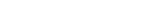
\includegraphics{ch07/figs/inductor-symbol}},
has no resistance; the resistor $R$ has no inductance. It is
this idealized circuit that we shall now analyze.

If the current $I$ in the circuit is changing at the rate $\der I/\der t$, an electromotive
force $L\der I/\der t$ will be induced, in a direction to oppose the
change. Also, there is the constant electromotive force $\emf_0$ of the
% p. 253
battery. If we define the positive current direction as the one in
which the battery tends to drive current around the circuit, then the
net electromotive force at any instant is $\emf_0 - L\der I/\der t$. This drives
the current $I$ through the resistor $R$. That is,
\begin{equation}
  \emf_0 - L\frac{\der I}{\der t} = RI
\end{equation}

We can also describe the situation in this way: The potential difference
between points $A$ and $B$, which we'll call the \emph{voltage across
the inductor}, is $L\der I/\der t$, with the upper end of the inductor positive
if $I$ in the direction shown is \emph{increasing}. The potential difference
between $B$ and $C$, the voltage across the resistor, is $RI$, with the upper
end of the resistor positive. Hence the sum of the voltage across the
inductor and the voltage across the resistor is $L\der I/\der t+RI$. This is
the same as the potential difference between the battery terminals,
which is $\emf_0$ (our idealized battery has no internal resistance). Thus
we have
\begin{equation}
  \emf_0 = L\frac{\der I}{\der t} + RI
\end{equation}
which is merely a restatement of Eq. 60.

Before we look at the mathematical solution of Eq. 60, 1et's predict
what ought to happen in this circuit if the switch is closed at $t = 0$.
Before the switch is closed, $I = 0$, necessarily. A long time after the
switch has been closed, some steady state will have been attained,
with current practically constant at some value $I_0$. Then and there-
after, $\der I/\der t\approx 0$, and Eq. 60 reduces to
\begin{equation}
  \emf_0 = RI_0
\end{equation}
The transition from zero current to the steady-state current $I_0$ cannot
occur abruptly at $t = 0$, for then $\der I/\der t$ would be infinite. In fact,
just after $t = 0$, the current $I$ will be so small that the second term
$RI$ in Eq. 60 can be ignored, giving
\begin{equation}
  \frac{\der I}{\der t} = \frac{\emf_0}{L}
\end{equation}
The inductance $L$ limits the rate of rise of the current.

What we now know is summarized in Fig. 7.24a. It only remains
to find how the whole change takes place. Equation 60 is a differential 
equation like some you have already met in Sec. 4.11 and in
% p. 254
Vol. 1, Chap. 6. Without further ado we can write down a solution
to Eq. 60 which satisfies our initial condition, $I = 0$ at $t = 0$.
\begin{equation}
  I = \frac{\emf_0}{R}\left(1-e^{-(R/L)t}\right)
\end{equation}

The graph in Fig. 7.24b shows the current approaching its asymptotic
value $I_0$ exponentially. The ``time constant'' of this circuit is
the quantity $L/R$. If $L$ is measured in henrys and $R$ in ohms, this
comes out in seconds, since $\zu{henrys} \sim \zu{vo1ts}/ (\zu{A}/\sunit)$, and
$\zu{ohms} \sim \zu{volts}/\zu{A}$.

What happens if we open the switch after the current $I_0$ has been
established, thus forcing the current to drop abruptly to zero? That
would make the term $L\der I/\der t$ negatively infinite! The catastrophe
can be more than mathematical. People have been killed opening
switches in highly inductive circuits. What happens generally is that
a very high induced voltage causes a spark or are across the open
switch contacts, so that the current continues after all. Let us instead
remove the battery from the circuit by closing a conducting
path \emph{across} the $LR$ combination, as in Fig. 7.25a, at the same time 
disconnecting the battery. We now have a circuit described by the
equation
\begin{equation}
  0 = L \frac{\der I}{\der t} +RI
\end{equation}
with the initial condition $I = I_0$ at $t = t_1$, where $t_1$ is the instant at
which the short circuit was closed. The solution is the simple exponential
decay function:
\begin{equation}
  I = I_0 e^{-(R/L)(t-t_1)}
\end{equation}
with the same characteristic time, $L/R$, as before.

\section{Energy stored in the magnetic field}
During the decay of the current described by Eq. 66 and Fig. 7.25b,
energy is dissipated in the resistor $R$. Since the energy $\der U$ dissipated
in any short interval $\der t$ is $RI^2 \der t$, the total energy dissipated after
the closing of the switch at time $t_1$ must be:
\begin{equation}
  U = \int_{t_1}^\infty RI^2\der t
    = \int_{t_1}^\infty RI_0^2e^{-(2R/L)(t-t_1)}\der t
\end{equation}
% p. 255
With the substitution $x = 2R(t - t_1)/L$ this is easily evaluated:
\begin{equation}
  U = RI_0^2\left(\frac{L}{2R}\right)\int_0^\infty e^{-x}\der x = \frac{1}{2}LI_0^2
\end{equation}

The source of this energy was the inductor with its magnetic field.
Indeed, exactly that amount of work had been done by the battery
to build up the current in the first place---over and above the energy
dissipated in the resistor between $t = 0$ and $t = t_1$, which was also
provided by the battery. To see that this is a general relation, note
that if we have an increasing current in an inductor, work must be
done to drive the current $I$ against the induced electromotive force
$L\der I/\der t$. So in time dt the work done is
\begin{equation}
  \der W = LI\frac{\der I}{\der t} \der t
         = LI\der I
         = \frac{1}{2}L\der(I^2)
\end{equation}
Therefore, we may assign a total energy
\begin{equation}
  U = \frac{1}{2}LI^2
\end{equation}
to an inductor carrying current $I$. With the eventual decay of this
current, that amount of energy will appear somewhere else.

It is natural to regard this as energy stored in the magnetic field
of the inductor, just as we have described the energy of a charged
capacitor as stored in its electric field. The energy of a capacitor
charged to potential difference $V$ is $\frac{1}{2}CV^2$, and is accounted for by
assigning to an element of volume $\der v$, where the electric field strength
is $E$, an amount of energy $(1/8\pi)E^2\der v$. It is pleasant, but hardly
surprising, to find that an exactly similar relation holds for the energy
stored in an inductor. That is, we can ascribe to the magnetic field
an energy density $(1/8\pi)B^2\der v$, and summing the energy of the whole
field will give the energy $\frac{1}{2}LI^2$.

To show how this works out in one case, we can go back to the
toroidal coil whose inductance $L$ we calculated in Sec. 7.8. We
found (Eq. 58)
\begin{equation}
  L = \frac{2N^2h}{c^2}\ln\left(\frac{b}{a}\right)
\end{equation}
The magnetic field strength $B$, with current $I$ flowing, was
\begin{equation}
  B = \frac{2NI}{cr}
\end{equation}
% p. 256
To calculate the volume integral of $B^2/8\pi$ we can use a volume element
consisting of the cylindrical shell sketched in Fig. 7.26, with
volume $2\pi rh\der r$. As this shell expands from $r = a$ to $r = b$, it sweeps
through all the space that contains magnetic field. (The field $B$ is
zero everywhere outside the torus, remember.)
\begin{equation}
  \frac{1}{8\pi}\int B^2\der v = \frac{1}{8\pi}\int_a^b\left(\frac{2NI}{cr}\right)^2 \: 2\pi rh\der r
        = \frac{N^2hI^2}{c^2} \ln\left(\frac{b}{a}\right)
\end{equation}
Comparing this result with Eq. 71, we see that, indeed,
\begin{equation}
  \frac{1}{8\pi}\int B^2\der v = \frac{1}{2}LI^2
\end{equation}

The more general statement, the counterpart of our statement for
the electric field in Eq. 1.36, is that the energy $U$ to be associated with
any magnetic field $B(x,y,z)$ is given by:
\begin{equation}
\boxed{
  U = \frac{1}{8\pi}\int_{\begin{matrix}\text{Entire}\\ \text{field}\end{matrix}} B^2\der v
}
\end{equation}
With $B$ in gauss and $v$ in cubic centimeters, $U$ in Eq. 75 will be given
in ergs. In Eq. 70, we may use practical units, henrys and amperes,
for $L$ and $I$, and then $U$ will be given in joules.

\section{``Something is missing''}

Let us review the relations between charges and fields. As we
learned in Chap. 2, a statement equivalent to Coulomb's law is the
differential relation
\begin{equation}
  \div\vc{E} = 4 \pi\rho
\end{equation}
connecting the electric charge density $\rho$ and the electric field $\vc{E}$. This
holds for moving charges as well as stationary charges. That is, $\rho$ can
be a function of time as well as position. As we emphasized in
Chap. 5, the fact that Eq. 76 holds for moving charges is consistent
with \emph{charge invariance}: No matter how an isolated charged particle
may be moving, its charge, as measured by the integral of $\vc{E}$ over a
surface surrounding it, appears the same in every frame of reference.

% p. 257

Electric charge in motion is electric current. Because charge is
never created or destroyed, the charge density $\rho$ and the current
density $\vc{J}$ always satisfy the condition
\begin{equation}
  \div\vc{J} = -\frac{\partial\rho}{\partial t}
\end{equation}
We first wrote down this ``Equation of Continuity'' as Eq. 4.9.

If the current density $\vc{J}$ is constant in time, we call it a stationary
current distribution. The magnetic field of a stationary current distribution
satisfies the equation
\begin{equation}
  \curl\vc{B} = \frac{4\pi}{c}\vc{J}
\end{equation}
We worked with this relation in Chap. 6.

Now we are interested in charge distributions and fields that are
changing in time. Suppose we have a charge distribution $\rho(x,y,z,t)$
with $\partial\rho/\partial t\ne 0$. For instance, we might have a capacitor which is
discharging through a resistor. According to Eq. 77, $\partial\rho/\partial t\ne 0$
implies
\begin{equation}
  \div\vc{J} \ne 0
\end{equation}
But according to Eq. 78, since the divergence of the curl of any
vector function is identically zero (see Prob. 2.15),
\begin{equation}
  \div\vc{J} = \frac{c}{4\pi}\div(\curl\vc{B}) = 0
\end{equation}
The contradiction shows that Eq. 78 \emph{cannot be correct} for a system
in which the charge density is varying in time. Of course, no one
claimed it was; a stationary current distribution, for which Eq. (78)
does hold, is one in which not even the current density $\vc{J}$, let alone the
charge density $\rho$, is time-dependent.

The problem can be posed in somewhat different terms by considering
the line integral of magnetic field around the wire carrying
charge away from the capacitor plate in Fig. 7.27. According to
Stokes' theorem,
\begin{equation}
  \int_C \vc{B}\cdot\der\bell = \int_S \curl\vc{B}\cdot\der\vc{a}
\end{equation}
The surface $S$ passes right through the conductor in which a current
$I$ is flowing. Inside this conductor, $\curl\vc{B}$ has a finite value,
namely $4\pi\vc{J}/c$, and the integral on the right comes out equal to $4\pi I/c$.
That is to say, if the curve $C$ is close to the wire and well away from
the capacitor gap, the magnetic field there is not different from the
% p. 258
field around any wire carrying the same current. Now the surface $S'$
in Fig. 7.28 is also a surface spanning $C$, and has an equally good
claim to be used in the statement of Stokes' theorem, Eq. 81.
Through this surface, however, there flows no current at all! 
Nevertheless, $\curl\vc{B}$ cannot be zero over all of $S'$ without violating Stokes'
theorem. Therefore, on $S'$, $\curl\vc{B}$ must depend on something other
than the current density $\vc{J}$.

We can only conclude that Eq. 78 has to be replaced by some
other relation, in the more general situation of changing charge 
distributions. Let's write instead
\begin{equation}
  \curl\vc{B} = \frac{4\pi}{c}\vc{J} + (?)
\end{equation}
and see if we can discover what (?) must be.

Another line of thought suggests the answer. Remember that the
transformation laws of the electromagnetic field, Eq. 6.58, are quite
symmetrical in $\vc{E}$ and $\vc{B}$. Now in Faraday's induction phenomenon
a \emph{changing magnetic field} is accompanied by an \emph{electric field}, in a
manner described by our Eq. 30:
\begin{equation}
  \curl\vc{E} = -\frac{1}{c}\frac{\partial\vc{B}}{\partial t}
\end{equation}
% p. 259
This is a local relation connecting the electric and magnetic fields in
empty space-charges are not directly involved. If symmetry with
respect to $\vc{E}$ and $\vc{B}$ is to prevail, we must expect that a changing electric
field can give rise to a \emph{magnetic field}. There ought to be an induction
phenomenon described by an equation like Eq. 30, but with
the roles of $\vc{E}$ and $\vc{B}$ switched. It will turn out that we need to change
the sign too, but that is all:
\begin{equation}
  \curl\vc{B} = \frac{1}{c}\frac{\partial\vc{E}}{\partial t}
\end{equation}

This provides the missing term that is called for in Eq. 82. To
try it out, write
\begin{equation}
  \curl\vc{B} = \frac{4\pi}{c}\vc{J} + \frac{1}{c}\frac{\partial\vc{E}}{\partial t}
\end{equation}
and take the divergence of both sides:
\begin{equation}
  \div(\curl\vc{B}) = \div\left(\frac{4\pi}{c}\vc{J}\right) + 
            \div\left(\frac{1}{c}\frac{\partial\vc{E}}{\partial t}\right)
\end{equation}
The left side is necessarily zero, as already remarked. In the second
term on the right we can interchange the order of differentiation with
respect to space coordinates and time. Thus
\begin{equation}
  \div\left(\frac{1}{c}\frac{\partial\vc{E}}{\partial t}\right)
   = \frac{1}{c}\frac{\partial}{\partial t}(\div\vc{E})
   = \frac{4\pi}{c} \frac{\partial\rho}{\partial t}
\end{equation}
by Eq. 76. The right-hand side of Eq. 85 now becomes
\begin{equation}
  \frac{4\pi}{c}\div\vc{J}+\frac{4\pi}{c}\frac{\partial\rho}{\partial t}
\end{equation}
which is zero by virtue of the continuity condition, Eq. 77.

The new term resolves the difficulty raised in Fig. 7.28. As charge
flows out of the capacitor, the electric field, which at any instant has
the configuration in Fig. 7.29, \emph{diminishes} in intensity. In this case,
$\partial\vc{E}/\partial t$ points opposite to $\vc{E}$. 
The vector function $\frac{1}{c}\frac{\partial\vc{E}}{\partial t}$ is represented
by the black arrows in Fig. 7.30.
With $\curl\vc{B} = \frac{4\pi}{c}\vc{J} + \frac{1}{c}\frac{\partial\vc{E}}{\partial t}$, the
integral of $\curl\vc{B}$ over S' now has the same value as it does over $S$.
On $S'$ the second term contributes everything; on $S$ the first term, the
term with $\vc{J}$, is practically all that counts.

% p. 260
% p. 261
\section{The displacement current}

Observe that the vector field $\frac{1}{c}\frac{\partial\vc{E}}{\partial t}$
appears to form a \emph{continuation}
of the conduction current distribution. Maxwell called it the \intro{displacement
current}, and the name has stuck although it no longer
seems very appropriate. To be precise, we can define a
``displacement current density" $\vc{J}_d$, to be distinguished from the conduction
current density $\vc{J}$, by writing Eq. 84 this way:
\begin{equation}
  \curl\vc{B} = \frac{4\pi}{c}(\vc{J}+\vc{J}_d)
\end{equation}
and defining $\vc{J}_d \equiv \frac{1}{4\pi}\frac{\partial\vc{E}}{\partial t}$.

We needed the new term to make the relation between current and
magnetic field consistent with the continuity equation, in the case
of conduction currents changing in time. If it belongs there, it
implies the existence of a new induction effect in which a changing
electric field is accompanied by a magnetic field. If the eff'ect is real,
why didn't Faraday discover it? For one thing, he wasn't looking
for it, but there is a more fundamental reason why experiments like
F araday's could not have revealed any new effects attributable to the
last term in Eq. 84. In any apparatus in which there are changing
electric fields, there are present at the same time conduction currents,
charges in motion. The magnetic field $\vc{B}$, everywhere around the
apparatus, is just about what you would expect those conduction
currents to produce. In fact, it is almost exactly the field you would
calculate if, ignoring the fact that the circuits may not be continuous,
you used the ``Biot-Savart'' formula, Eq. 6.38, to find the contribution
of each conduction current element to the field at some point in space.

Consider, for example, the point $P$ in the space between our discharging
condenser plates, Fig. 7.31. Each element of conduction
current, in the wires and on the surface of the plates, contributes to
the field at $P$, according to the Biot-Savart formula. Must We include
also the elements of ``displacement current'' $\vc{J}_d$? The answer is rather
surprising. We \emph{may} include $\vc{J}_d$; but if we are careful to include the
entire displacement current distribution, its net effect will be \emph{zero} for
relatively slowly varying fields.

To see why this is so, notice that the vector function $\vc{J}_d$, indicated
by the black arrows in Fig. 7.30, has the same form as the electric
field $\vc{E}$ in Fig. 7.29. This electric field is practically an electrostatic
field, except that it is slowly dying away. We expect therefore that
its curl is practically zero which would imply that $\curl\vc{J}$ must be
% p. 262
practically zero. More precisely, we have $\curl\vc{E} = -\frac{1}{c}\frac{\partial\vc{B}}{\partial t}$ and
with the displacement current $\vc{J}_d=\frac{1}{4\pi}\frac{\partial\vc{E}}{\partial t}$,
we get, by interchanging the order of differentiation,
\begin{equation}
  \curl \vc{J}_d = \frac{1}{4\pi}\curl\left(\frac{\partial\vc{E}}{\partial t}\right)
        = \frac{1}{4\pi}\frac{\partial}{\partial t}(\curl\vc{E})
        = -\frac{1}{4\pi c}\frac{\partial^2\vc{B}}{\partial t^2}
\end{equation}
This will be negligible for sulficiently slow changes in field. We
may call a slowly changing field \emph{quasi-static}.\index{quasi-static field}
Now if $\vc{J}_d$ is a vector
field without any curl, it can be made up, in the same way that the
electrostatic field can be made of the fields of point charges, by superposing
radial currents flowing outward from point sources or in
toward point ``sinks'' (Fig. 7.32). But the magnetic field of any
\emph{radial}, symmetrical current distribution, calculated \emph{\`a la} Biot-Savart,
must be zero by symmetry, for there is no unique direction anywhere,
except the radial direction itself.

In the \emph{quasi-static} field, then, the conduction currents alone are
the only \emph{sources} needed to account for the magnetic field. In other
words, if Faraday had arranged something like Fig. 7.31, and had
been able to measure the magnetic field at $P$, by using a compass
needle say, he would not have been surprised. He would not have
needed to invent a displacement current to explain it.

% p. 263

To see this new induction effect, we need rapidly changing fields.
In fact, we need changes to occur in the time it takes light to cross
the apparatus. That is why the direct demonstration had to wait for
Hertz, whose experiment came many years after the law itself had
been worked out by Maxwell.

\section{Maxwell's equations}

James Clerk Maxwell, after immersing himself in the accounts of
Faraday's electrical researches, set out to formulate mathematically
a theory of electricity and magnetism. Maxwell could not exploit
re1ativity---that came fifty years later. The electrical constitution
of matter was a mystery, the relation between light and electromagnetism
unsuspected. Many of the arguments that we have used to
make our next step seem obvious were unthinkable then. 
Nevertheless, as Maxwell's theory developed, the term we have been 
discussing, $\partial\vc{E}/\partial t$, appeared quite naturally in his formulation. He called
it the ``displacement current.'' Maxwell was concerned with electric
fields in solid matter as well as in vacuum, and when he talks about
a ``displacement current'' he is often including some 
charge-in-motion, too. We'll clarify that point in Chap. 9 when we study electric
fields in matter. Indeed, Maxwell thought of space itself as a
medium, the ``aether,'' so that even in the absence of solid matter the
displacement current was occurring in something. But never mind---
his mathematical equations were perfectly clear and unambiguous,
and his introduction of the displacement current was a \emph{theoretical}
discovery of the first rank. 

Maxwell's description of the electromagnetic field was essentially
complete. We have arrived by different routes at various pieces of it,
which we shall now assemble in the form traditionally called
\intro{Maxwell's equations}:
\begin{framed}
\begin{align}
\begin{split}
  \curl\vc{E} &= -\frac{1}{c}\frac{\partial\vc{B}}{\partial t} \\
  \curl\vc{B} &= \frac{1}{c}\frac{\partial\vc{E}}{\partial t} + \frac{4\pi}{c}\vc{J} \\
  \div\vc{E} &= 4\pi\rho \\
  \div\vc{B} &= 0
\end{split}  
\end{align}
\end{framed}
These are written for the fields in vacuum, in the presence of electric
charge of density $\rho$ and electric current, that is, charge-in-motion,
of density $\vc{J}$.

% p. 264

The first equation is Faraday's \emph{law of induction}. The second
expresses the dependence of the magnetic field on the \emph{displacement
current} density, or rate-of-change of electric field, and on the \emph{conduction
current density}, or rate-of-motion of charge. The third
equation is equivalent to Coulomb's law. The fourth equation states
that there are no sources of magnetic field \emph{except} currents. We shall
have more to say about this aspect of Nature in Chap. 10.

Notice that the lack of symmetry in these equations, with respect
to $\vc{B}$ and $\vc{E}$, is entirely due to the presence of electric charge and 
electric conduction current. In empty space, the terms with $\rho$ and $\vc{J}$ are
zero, and Maxwell's equations become
\begin{framed}
\begin{align}
\begin{split}
  \curl\vc{E} &= -\frac{1}{c}\frac{\partial\vc{B}}{\partial t} \qquad
  \div\vc{E} = 0 \\
  \curl\vc{B} &= \quad \frac{1}{c}\frac{\partial\vc{E}}{\partial t} \qquad
  \div\vc{B} = 0
\end{split}  
\end{align}
\end{framed}

Here the displacement current term is all-important. Its presence,
along with its counterpart in the first equation, implies the possibility
of \intro{electromagnetic waves}. Recognizing that, Maxwell went on to
develop with brilliant success an electromagnetic theory of light.
You will be exploring the physics of waves, and of light waves in
particular, in Vol. III. We can show right now that an electromagnetic
disturbance traveling at speed $c$ is compatible with Maxwell's
equations. To do this, we shall describe a very simple set of electric
and magnetic fields which represent a traveling disturbance, and
then we shall show that these fields satisfy all the equations in the
box, Eqs. 91.

At the instant of time $t = 0$, there exists, we suppose, an electric
field in the region between the planes $y = 0$ and $y = 2a$. This field $\vc{E}$
has a $z$ component only, and its $z$ component depends only on $y$, in
the following manner at time $t=0$:
% FIXME - kludgy use of qquads to line things up
\begin{align}
\begin{split}
  E_z &= E_0\frac{y}{a}        \qquad\qquad\qquad (0\le y \le a) \\
  E_z &= E_0\left(\frac{2a-y}{a}\right) \qquad (a \le y \le 2a)
\end{split}
\end{align}
As indicated in Fig. 7.33a, this describes a ``gable''-shaped distribution
of field strength, maximum in the center at $y = a$ and falling off
linearly to zero at $y = a$ and $y = 2a$. For given $y$, the field is the
same at all $x$ and $z$. That is, we have electric field throughout an
% p. 265
% p. 266
infinite slab, although in the figure we show field vectors on the $y$ axis
only. The shaded patches marked I and II lie within this slab.
Everywhere outside the slab, that is, for $y < 0$ and $y > 2a$, the electric
field is zero at this instant of time. At the same time a magnetic
field $\vc{B}$ exists in this slab of space. It has an $x$ component only,
given at $t=0$ by:
% FIXME - kludgy use of qquads to line things up
\begin{align}
\begin{split}
  B_x &= B_0\frac{y}{a}        \qquad\qquad\qquad (0\le y \le a) \\
  B_x &= B_0\left(\frac{2a-y}{a}\right) \qquad (a \le y \le 2a)
\end{split}
\end{align}

We simply invented this field. Let us now command the field
configuration to travel in the $y$ direction with speed $c$, while preserving
its shape. We can do that by writing out orders as follows:
\linebreak[4]\noindent\emph{Region I ($ct \le y \le ct+a$):}
\begin{align}
\begin{split}
  E_z &= E_0 \left(\frac{y-ct}{a}\right) \\
  B_x &= B_0 \left(\frac{y-ct}{a}\right) \\
\end{split}
\end{align}
\emph{Region II ($ct+a \le y \le ct+2a$):}
\begin{align}
\begin{split}
  E_z &= E_0 \left(\frac{2a-y+ct}{a}\right) \\
  B_x &= B_0 \left(\frac{2a-y+ct}{a}\right) \\
\end{split}
\end{align}
This describes the situation as we see it in Fig. 7.33b or at any other
time $t$. The region containing field is simply displaced to the right
by a distance $ct$. Within regions I and II, both $\vc{E}$ and $\vc{B}$ have the same
form as before. Our equations, then, describe a traveling configuration
of electric and magnetic fields, but can such fields exist? To
answer that, we must see if $\vc{E}$ and $\vc{B}$, as given by Eqs. 94 and 95, satisfy
Maxwell's equations.

Beginning with the divergence equations, it is easy to see that
$\div\vc{E} = 0$ and $\div\vc{B} = 0$. (Obviously $\partial E_z/\partial z = 0$ and the other
components of $\vc{E}$ are themselves zero.) But $\curl\vc{E}$ is not zero.
Instead, its value is:
\begin{align}
\begin{split}
  \text{In \emph{Region I}:}  \qquad & \grad\times\vc{E} = \xhat \frac{\partial E_z}{\partial y} 
                                                      = \frac{E_0}{a} \xhat \\
  \text{In \emph{Region II}:} \qquad & \grad\times\vc{E} = \xhat \frac{\partial E_z}{\partial y} 
                                                      = -\frac{E_0}{a} \xhat 
\end{split}
\end{align}

In the same way we calculate $\grad\times\vc{B}$:
\begin{align}
\begin{split}
  \text{In \emph{Region I}:}  \qquad & \grad\times\vc{B} = -\zhat \frac{\partial B_x}{\partial y} 
                                                      = -\frac{B_0}{a} \zhat \\
  \text{In \emph{Region II}:} \qquad & \grad\times\vc{B} = -\zhat \frac{\partial B_x}{\partial y} 
                                                      = \frac{B_0}{a} \zhat 
\end{split}
\end{align}

The partial derivatives with respect to $t$ are:
\begin{align}
\begin{split}
  \text{In \emph{Region I}:}  \qquad 
             \frac{\partial\vc{E}}{\partial t} = -\frac{c}{a}E_0\zhat
           \qquad & \qquad \frac{\partial\vc{B}}{\partial t} = -\frac{c}{a}B_0\xhat \\
  \text{In \emph{Region II}:}  \qquad 
             \frac{\partial\vc{E}}{\partial t} = \frac{c}{a}E_0\zhat
           \qquad & \qquad \frac{\partial\vc{B}}{\partial t} = \frac{c}{a}B_0\xhat 
\end{split}
\end{align}
The fields will satisfy the ``induction'' equations in region I, then, if
% FIXME - why does intertext make these equations end up flush left?
\begin{align}
\begin{split}
  \frac{E_0}{a}\xhat &= -\frac{1}{c}\left(-\frac{c}{a}B_0\xhat\right) \\
\intertext{and}
  -\frac{B_0}{a}\zhat &= \frac{1}{c}\left(-\frac{c}{a}E_0\zhat\right) 
\end{split}
\end{align}
Indeed, these are satisfied provided $E_0 = B_0$. The equations lead
to exactly the same requirement for the fields in region II. Exactly
at the peak of the gable, and also at each end, there are mathematical
singularities in the assumed fields. To be sure that the field equations
are satisfied \emph{everywhere}, we must see that there is no trouble at these
points. There is none, because $\vc{E}$ and $\vc{B}$ are \emph{continuous} there. (An
abrupt jump. or discontinuity, in $\vc{E}$ or $\vc{B}$ would not be possible in
empty space.) Thus the particular electromagnetic field we have
described, which \emph{does} represent a traveling wave, \emph{does} satisfy all the
field equations, if the electric field, in statvolts/cm, is everywhere
equal to the magnetic field strength, at the same time and place. It is
essential that $\vc{E}$ and $\vc{B}$ be perpendicular to one another and to the
direction of travel---otherwise the field equation could not have been
satisfied.

Our traveling ``gable'' may strike you as a rather special kind of
wave. In fact, this simple example reveals all that is essential about
\emph{any} plane electromagnetic wave! We need only think of 
\emph{superposition}. As we have frequently emphasized, the equations of the
electromagnetic field are linear. If two sets of fields satisfy Maxwell's
equations, so does their sum. We can have any number of our
``gable'' fields traveling through space, in the same or different direc-
tions. (Naturally, the fields don't care how the axes are oriented---
% p. 268
any other direction is as good as the $y$ axis.) Fig. 7.34 suggests some
of the waves you could make with ``gables.'' It is pretty obvious that
\emph{any} function could be approximated as closely as desired by superposing
``gables.'' Therefore, what we have learned about the gable
wave must apply to any wave in which $\vc{E}$ and $\vc{B}$ are functions only
of the coordinate in the direction of travel. These general facts are:
\begin{enumerate}[(i)]
\item The disturbance travels with speed $c$, with unchanging form. 
\item $\vc{E}$ and $\vc{B}$ are perpendicular to each other and to the direction
    of travel, with the vector $\vc{E}\times\vc{B}$ always pointing in the
    direction of the travel, as it does in our example.
\item At a given point and time, $E = B$.
\end{enumerate}

An electromagnetic field with these properties transforms in a
simple and satisfying way when we change coordinate systems. In
Chap. 6 we derived formulas for the Lorentz transformation of the
electric and magnetic fields (Eq. 6.58). Let's use the results of
Prob. 6.11, which were based on those equations, according to which
the two scalar quantities, $E^2 - B^2$ and $\vc{E}\cdot\vc{B}$ remain invariant in a
transformation to another inertial frame. In this case, since $E = B$
at any point, the invariant quantity $E^2 - B^2$ has the value zero. Also.
because $\vc{E}$ is perpendicular to $\vc{B}$, the other invariant $\vc{E}\cdot\vc{B}$ is zero. It
follows that in any other frame the transformed fields $\vc{E}'$ and $\vc{B}'$ must
be equal to each other in magnitude and perpendicular in direction.
A light wave looks like a light wave in any frame of reference.
